% Определение класса для файла
\documentclass[12pt, times]{article} % размер 12, шрифт Times New Roman

% Подключение файла с настройками и подключенными пакетами
% Макет страницы
\usepackage[a4paper, left=3.5cm, right=1.5cm, top=2cm, bottom=2cm]{geometry} % подключает пакет geometry для управления размерами страницы
\usepackage[onehalfspacing]{setspace} % 1.5 интервал
\usepackage{indentfirst} % добавляет отступ для абзаца после секции

% Настрока заголовков и подзаголовков для оглавления
\usepackage{titlesec}

% Настройка \section: шрифт 14pt, выравнивание по центру
\titleformat{\section}
  {\normalfont\fontsize{14}{16}\selectfont\bfseries\centering} % стиль шрифта заголовка
  {} % без номера в тексте, но номер будет в ToC
  {0pt} % расстояние между номером и заголовком
  {} % код перед названием секции
% Отступ слева = абзацный отступ, сверху = 2 строки, снизу = 1 строка
\titlespacing*{\section}
  {0pt} % левый отступ не нужен
  {2ex} % отступ сверху
  {1ex} % отступ снизу

% Настройка \subsection: шрифт 12pt, выравнивание по абзацу
\titleformat{\subsection}
  {\normalfont\fontsize{12}{14}\selectfont\bfseries} % стиль шрифта подзаголовка
  {} % без номера в тексте, но будет номер в ToC
  {0pt} % расстояние между номером и заголовком
  {} % код перед названием

\titlespacing*{\subsection}
  {\parindent} % левый отступ как у абзаца
  {3ex} % отступ сверху
  {1ex} % отступ снизу

% Настройка \subsubsection: шрифт 12pt, выравнивание по абзацу
\titleformat{\subsubsection}
  {\normalfont\fontsize{12}{14}\selectfont\bfseries} % стиль шрифта подзаголовка
  {} % без номера в тексте, но будет номер в ToC
  {0pt} % расстояние между номером и заголовком
  {} % код перед названием

\titlespacing*{\subsubsection}
  {\parindent} % левый отступ как у абзаца
  {3ex} % отступ сверху
  {1ex} % отступ снизу

% Настройки внутри списков
\usepackage{enumitem}

% Добавляем точки в оглавление
\usepackage{tocloft}
\renewcommand{\cftsecleader}{\cftdotfill{\cftdotsep}} % добавляем точки
\renewcommand{\cftdotsep}{1} % плотность точек

% Кодировка и поддержка кириллицы
\usepackage[utf8]{inputenc} % позволяет использовать текст в кодировке UTF-8
\usepackage[T2A]{fontenc} % поддержка русских шрифтов (кириллица)
\usepackage[english, russian]{babel} % включение правил типографики для английского языка (переносы, заголовки и т.д.)

% Кавычки и цитаты
\usepackage{csquotes} % поддержка корректного форматирования кавычек и цитат (особенно важно при использовании biblatex)

% Вставка изображений
\usepackage{graphicx} % позволяет вставлять и масштабировать изображения (\includegraphics)

%\begin{figure}[htbp] % here, top, bottom, page
%    \centering
%    \includegraphics[width=0.8\textwidth]{имя_файла.png}
%    \caption{Подпись к рисунку}
%    \label{fig:example}
%\end{figure}

% Указание папки для поиска изображений
\graphicspath{{images/}}

% Таблицы
\usepackage{array} % расширенные возможности для работы с таблицами
\usepackage{tabularx} % автоматический подбор ширины столбцов

\usepackage{multirow} % настройка для множественных строк
\renewcommand{\arraystretch}{1.0} % размер между строк таблиц, 1.0 по умолчанию

\usepackage{longtable} % позволяет создавать таблицы, которые переносятся на следующие страницы
\usepackage{etoolbox} % нужен для двух следующих команд
\AtBeginEnvironment{table}{\fontsize{10}{10}\selectfont} % для изменения размера шрифта меняем первое значение в {}
\AtBeginEnvironment{longtable}{\fontsize{10}{10}\selectfont} % для изменения размера шрифта меняем первое значение в {}

% Математические выражения
\usepackage{amsmath, amssymb} % расширенные математические окружения; дополнительные математические символы

% Ссылки
\usepackage[
    colorlinks=true, % включение цвета для ссылок
    linkcolor=black, % цвет оглавления
    urlcolor=blue, % цвет url-ссылок в тексте и библиографии
    citecolor=black % цвет для текста в цитатах
]{hyperref} % добавляет активные гиперссылки на разделы, рисунки, библиографию и внешние URL

% Подписи к картинкам и таблицам
\usepackage[justification=centering]{caption} % более гибкое управление подписями к рисункам и таблицам
\captionsetup[table]{labelfont=bf, textfont=bf} % textfont=normalfoint для обычного шрифта в тексте таблиц
\captionsetup[figure]{labelfont=bf, textfont=bf} % textfont=normalfoint для обычного шрифта в тексте картинок
\usepackage{subcaption} % позволяет делать несколько подрисунков с подписями (a), (b), ...

% Библиография
\usepackage[backend=biber, style=gost-numeric, autolang=other, sorting=none]{biblatex}
% использование biber для обработки ссылок
% ГОСТ-стиль нумерованной библиографии
% язык библиографии подбирается автоматически, нужно поле langid = {russian} или langid = {english} в .bib файле
\addbibresource{bib/bibliography.bib}
% заменим ; на запятую между несколькими ссылками
\renewcommand*{\multicitedelim}{\addcomma\space}

\begin{document}

% Титульный лист
\newpage
\begin{titlepage}

\begin{center}
    САНКТ-ПЕТЕРБУРГСКИЙ ГОСУДАРСТВЕННЫЙ УНИВЕРСИТЕТ \\КАФЕДРА ГЕНЕТИКИ И БИОТЕХНОЛОГИИ
    \vspace{5cm}

    % Автор
    \textbf{Васильев Артем Викторович \\Выпускная квалификационная работа}
    \vspace{1cm}

    % Название работы
    ``Эволюционные особенности структуры гена \\\textit{Nxf1} (nuclear export factor) у животных``
\end{center}

\vfill

\begin{flushright}
    Научный руководитель: \\к.б.н., доцент, кафедра генетики и биотехнологии, \\Голубкова Елена Валерьевна \\
    \vspace{1cm}
    Рецензент: \\заведующая лабораторией, ведущий научный сотрудник, \\лаборатория эволюционной геномики и палеогеномики, ЗИН, \\к.б.н., с.н.с., \\Абрамсон Наталья Иосифовна
\end{flushright}

\vfill

\begin{center}
    Санкт-Петербург \\2025
\end{center}

\end{titlepage}

\setcounter{page}{2} % изменение номера СЛЕДУЮЩЕЙ страницы


% Аннотация
% \input{chapters/annotation}

% Оглавление
\newpage
\renewcommand{\contentsname}{\centerline{\large Оглавление}}
\tableofcontents


% Список использованных сокращений
% \input{chapters/abbreviations}

% Введение
% \clearpage
\section{Введение}

Для большинства генов высших эукариот характерна мозаичная структура, в составе которой выделяют кодирующие участки экзоны и некодирующие - интроны.
В процессе созревания транскрипта интроны, как правило, вырезаются сплайсингом, и из ядра выходят мРНК, лишенные интронных последовательностей.
Однако альтернативный сплайсинг позволяет получать несколько различных зрелых мРНК из одной пре-мРНК, что значительно расширяет протеом без увеличения числа генов.

Особый интерес представляют транскрипты, сохраняющие интрон (intron retention, IR): в таких первичных транскриптах интрон, обычно несущий преждевременный стоп-кодон, остается невырезанным, образуя устойчивую вторичную структуру, которая препятствует распознаванию факторами нонсенс-опосредованного распада (nonsense mediated mRNA decay, NMD) и впоследствии обеспечивает синтез укороченного, но функционально значимого белка~\cite{Mamon2019}.

Однако, несмотря на наличие специфического механизма, среди различных групп, эволюционно далеких друг от друга, описаны случаи существования транскриптов с сохраненным интроном.
Отдельно можно выделить модельный объект \textit{Drosophila melanogaster} и человека, для которых известно семейство генов \textit{Nxf} (nuclear export factor), в котором нас заинтересовал ген \textit{Nxf1}.
Данный ген кодирует белок, являющийся основным транспортером мРНК из ядра в цитоплазму.

У гена \textit{Nxf1} (nuclear export factor 1), кодирующего основной транспортер мРНК из ядра в цитоплазму, существует так называемая ``консервативная кассета``, которая включает два коротких экзона (110 и 37 нуклеотидов в каноническом варианте) и ``кассетный`` интрон между ними.
Названия сформулированы нашей научной группой.
Эта структура сохраняется также и у представителей других филогенетических групп: благодаря образованию специфической вторичной структуры или наличию в последовательности интрона специфических последовательностей, например конститутивного транспортного элемента (constitutive transport element, CTE), транскрипт, содержащий преждевременный стоп-кодон, избегает NMD и кодирует укороченную форму белка.

Анализ подобных транскриптов показал, что консервативные элементы ``кассеты`` \textit{Nxf1} специфичны для разных клад организмов, а интрон-содержащие транскрипты формируют уникальные вторичные структуры, что подчеркивает эволюционную и функциональную значимость интронов.

Научная новизна работы заключается в сравнительном анализе структуры гена \textit{Nxf1} у представителей различных филогенетических групп, данных по которым ранее не было, с целью выявления закономерностей эволюции нуклеотидной и белковой последовательности гена \textit{Nxf1}.
В бакалаврской работе было показано, что ``консервативная кассета`` сохраняет свойства внутри артропод, особенно внутри семейства Drosophilidae, однако вопрос о степени консервативности и специфике структурных элементов у более широкого круга организмов остается открытым.
Помимо сравнительного анализа последовательностей, важной частью исследования является построение вторичных структур интрон-содержащих транскриптов и выявление консервативных мотивов внутри интрона, способствующих его сохранению и избеганию нонсенс-опосредованного распада.


\subsection{Цель работы}

Изучить структуру гена \textit{Nxf1} у представителей разных филогенетических групп животных для выявления эволюционных закономерностей и особенностей ``кассетной`` структуры, а также проанализировать вторичные структуры интрон-содержащих транскриптов.


\subsection{Задачи}

\begin{enumerate}[left=\parindent]
  \item Найти нуклеотидные и аминокислотные последовательности гена \textit{Nxf1} у различных групп животных.
  \item Произвести поиск ``консервативной каасеты`` в нуклеотидной последовательности гена у найденных организмов.
  \item Выполнить анализ структуры, сравнить полученные последовательности между собой.
  \item Выявить и охарактеризовать консервативные участки ``кассетного`` интрона и прилегающих экзонов у видов из исследуемых таксонов.
  \item Провести анализ вторичной структуры интрон-содержащих транскриптов и оценить консервативные мотивы внутри интрона, потенциально способствующие его сохранению.
\end{enumerate}


% Обзор литературы
%%\clearpage
%\section{Обзор литературы}
%
%\subsection{Механизмы усложнения организации генома}
%
%Помимо стандартного варианта созревания РНК путем сохранения экзонов и сплайсосомного вырезания интронов из первичного транскрипта, существуют варианты, отличающиеся от канонического.
%Одним из таких вариантов является альтернативный сплайсинг - основной источник транскрипционной изменчивости, когда одному гену может соответствовать несколько транскриптов.
%Кроме общеизвестного ``удержания интрона`` (intron retention (IR)), важно обозначить такой процесс, как альтернативное полиаденилирование, так как оно также оказывает прямое влияние на вариативность транскриптов~\cite{Mamon2019}.
%
%Альтернативный сплайсинг (alternative splicing (AS)) достаточно распространен у эукариот.
%Данный механизм способствует увеличению белкового разнообразия у организма.
%Выделяют следующие типы альтернативного сплайсинга: т.н. ``пропуск экзонов``; вариант, когда используются наборы из нескольких экзонов, расположенных рядом друг с другом и  формирующих кассеты, при этом во время сплайсинга выбирается только один из нескольких экзонов в каждой из кассет; также могут использоваться различные 5'- и 3'-сайты сплайсинга в интронах или экзонах, выбор которых зависит от цис- и транс-действующих факторов, необходимых для формирования сплайсосомы~\cite{Mamon2019}.
%
%``Удержание интрона`` является одним из вариантов альтернативного сплайсинга, который распространен у млекопитающих.
%Данный механизм увеличивает сложность транскриптома~\cite{Schmitz2017}, но часто в интронах присутствуют кодоны преждевременной терминации (premature termination codons (PTCs)) внутри основной открытой рамки считывания.
%В результате возможно 2 исхода: нонсенс-опосредованный распад мРНК с сохраненным интроном или продукция укороченных белков~\cite{Mamon2019}.
%Именно эти варианты интересуют нас больше всего.
%Такие мРНК с оставшимся интроном дают альтернативные формы белков, а значит являются источником функционального разнообразия генных продуктов, что демонстрирует важность интронов как структурной единицы гена.
%Для разных организмов показано, что наличие такой мРНК с интроном для гена \textit{Nxf1} является консервативным признаком~\cite{Mamon2013}, о чем речь пойдет далее.
%
%
%\subsection{Значимость интронов}
%
%Интроны делят на 3 группы: I, II, III.
%Интроны I и II группы обнаруживаются в геномах некоторых бактерий и органелл.
%Интроны I группы также обнаружены в рибосомных РНК (рРНК) ядер протистов и грибов.
%Эти две группы имеют разные структуры РНК, которые облегчают их активность самосплайсинга.
%Они также содержат внутренние открытые рамки считывания (open reading frame (ORF)), которые облегчают как удаление интронов из транскриптов РНК, так и распространение интронов на безинтронные сайты посредством обратной транскрипции~\cite{Roy2006}.
%Третья же группа интронов – сплайсосомные интроны – найдены в ядерных геномах всех охарактеризованных эукариот.
%Обычно они не имеют открытых рамок считывания и их удаление происходит с помощью сплайсосомы~\cite{Jurica2013}.
%
%К непосредственным функциям интронов можно отнести следующее.
%Во-первых, это положительная регуляция экспрессии генов.
%Впервые данное явление было продемонстрировано очень давно в эксперименте с использованием конструкций вируса SV40, где показали, что количество белка было значительно снижено без его интронов~\cite{Gruss1979}.
%В последующем это было также показано на дрожжах и млекопитающих~\cite{Juneau2006}.
%
%Во-вторых, можно отнести регуляцию нонсенс-опосредованного распада мРНК, который был упомянут при описании удержания интрона.
%Обычно NMD описывают, как механизм надзора у эукариот, который избирательно удаляет мРНК, содержащие ошибочно сгенерированные PTCs~\cite{Jo2015}.
%Однако, есть доказательства в пользу того, что интроны, расположенные в 5'- или 3'-нетранслируемых областях (untranslated region (UTR)), играют важную роль в контроле NMD-чувствительности транскриптов~\cite{Kalyna2012}.
%
%В-третьих, интроны могут быть связаны с транспортом мРНК.
%Раньше считалось, что сплайсированные транскрипты быстрее экспортируются из ядра в цитоплазму, однако были и противоречивые исследования~\cite{Jo2015}.
%Один из относительно недавних экспериментов с использованием флуоресцентной гибридизацией in situ (FISH) показал, что несущие интроны транскрипты преимущественно расположены в цитоплазме~\cite{Valencia2008}, что сильнее подвергает сомнению высказанные ранее гипотезы и требует их пересмотра.
%
%Помимо перечисленных функций есть также предположение о том, что часть последовательностей концов интронов может быть ответственна за истощение нуклеосом в интронах путем отталкивания нуклеосом в сторону экзонов~\cite{Schwartz2009}.
%Это позволяет задуматься о роли интронов в сборке хроматина.
%
%Стоит отметить порядковое положение интронов в гене.
%Больше всего внимание привлекает первый интрон среди всех интронов гена, обычно именно он обладает особыми функциональными характеристиками~\cite{Jo2015}.
%Например, первый интрон гена \textit{oskar} Drosophila играет важную роль в правильной цитоплазматической локализации некоторых мРНК~\cite{Siemens2004}.
%
%Длина интронов также является важной характеристикой.
%Есть предположение о том, что длинные интроны повышают эффективность естественного отбора, устраняя интерференцию Хилла-Робертсона~\cite{Comeron2008}.
%
%В одной из работ десятилетней давности на дрожжах \textit{Saccharomyces cerevisiae} наблюдали, как короткие ORF могут эволюционировать в настоящие функциональные гены посредством своего рода непрерывного эволюционного процесса~\cite{Carvunis2012}.
%Это позволило предположить, что интроны могут стать источником новых генов.
%
%В наше время активно используется метод полногеномного поиска ассоциаций, сокращенно GWAS – genome-wide association study.
%В основе метода лежит сравнительный анализ однонуклеотидных вариантов (single-nucleotide variant (SNV)), а точнее участков в геноме, которые схожи между собой по этим однонуклеотидным заменам, между индивидуумами~\cite{Smith2019}.
%Примечательно, что при картировании аллелей, ассоциированных с какими-то заболеваниями, место картирования соответствует именно интронным областям~\cite{Welter2014}.
%Данный факт является очередным подтверждением важности изучения интронов.
%
%
%\subsection{Семейство генов \textit{Nxf}, общая характеристика}
%
%Принимая во внимание все выше сказанное, можно перейти к описанию основного объекта, на который направлено данное исследование.
%Перед этим стоит сказать несколько вводных слов про само семейство.
%
%Семейство генов \textit{Nxf} (nuclear export factor) было названо в честь функции универсального гена \textit{Nxf1}, продукт которого ответственен за ядерно-цитоплазматический транспорт большинства мРНК.
%Гены данного семейства обнаружены у всех эукариотических организмов группы Opisthokonta и характеризуются эволюционной консервативностью~\cite{Mamon2013}.
%
%Геномы различных грибов имеют лишь один ген-представитель этого семейства, растения и некоторые простейшие вовсе их лишены.
%Животные, как правило, имеют от двух до пяти паралогичных генов~\cite{Mamon2013}.
%
%Характерной особенностью для гена Nxf1 является существование транскриптов с невырезанным гомологичным интроном.
%Особое внимание выделяется консервативному блоку, состоящему из последовательно идущих экзонов размером 110 п.н. и 37 п.н., а также интрону, который находится между ними и который принято называть ``кассетным``~\cite{Mamon2013}.
%Соответственно, сам блок из трех единиц мы будем называть ``консервативной кассетой``.
%
%Среди животных, для которых есть данные про семейство генов Nxf, были выявлены 3 таксономические группы, и в каждой из них кассетный интрон имеет определенные характеристики~\cite{Mamon2013}.
%
%К первой группе относятся позвоночные, для них характерен интрон, находящийся между 10-м и 11-м экзонами в гене \textit{Nxf1}.
%В интроне позвоночных выявили 4 участка протяженной гомологии: 1) 5´-концевая последовательность; 2) фрагмент, содержащий конститутивный транспортный элемент (constitutive transport element (СТЕ), характерный для ретровирусов; 3) третий консервативный участок; 4) 3´-концевая последовательность~\cite{Mamon2013}.
%
%Ко второй группе принадлежат дрозофилиды с кассетным интроном 5-м в генах \textit{Nxf1}.
%Несмотря на отсутствие участков протяженной гомологии, что характерно для позвоночных, у разных видов Drosophilidae есть схожая черта – две протяженные последовательности, обогащенные аденином (А).
%Предполагается, что вторичная структура транскриптов с сохраненным интроном, образовавшаяся за счет наличия этих последовательностей, способствует их сохранению~\cite{Mamon2013}.
%
%В последнюю группу включены нематоды с интроном 5-м или 6-м.
%Его размер на порядок меньше, а участки протяженной гомологии не обнаружены.
%Однако, внутри группы есть общее сходство – это повышенное содержание тимина (Т), что отличает данную группу организмов от остальных~\cite{Mamon2013}.
%
%Как уже упоминалось ранее, важной особенностью для генов Nxf1 у позвоночных и дрозофилид является способность к образованию сложных вторичных структур, которая может играть существенную роль в пост-транскрипционной судьбе транскрипта~\cite{Golubkova2012}.
%Помимо этого, все же главной особенностью, кроме сохраненного интрона в транскрипте, становится наличие в этом сохранившемся интроне преждевременного стоп-кодона, но мРНК избегает нонсенс-опосредованного распада, и в итоге возможно образование укороченного белка.
%Перейдем к подробному рассмотрению гена \textit{Nxf1}.
%
%
%\subsection{Структура и функции Nxf1 (гена и белка)}
%
%Первоначально белок Nxf1 у людей был идентифицирован как потенциальный цитоплазматический кофактор для Tip (белок, взаимодействующий с тирозинкиназой), кодируемый вирусом герпеса saimiri, и был назван TAP (Tip-associated protein, или белок, ассоциированный с Tip)~\cite{Yoon1997}.
%Позже было показано, что ТАР участвует в ядерно- цитоплазматическом транспорте несплайсированной или частично сплайсированной РНК ретровирусов.
%TAP напрямую распознает только одну последовательность – CTE, которая была первоначально обнаружена в РНК ретровирусов~\cite{Zolotukhin2001}.
%Мы предполагаем, что функцию CTE у дрозофилид выполняет образуемая благодаря сохранению интрона вторичная структура.
%На данный момент наилучшее представление о гене \textit{Nxf1} есть для дрозофилид и млекопитающих.
%Рассмотрим функцию и организацию данного гена, а также белковые домены для \textit{Drosophila melanogaster} и \textit{Homo sapiens}.
%
%Nxf1 имеет модульную доменную организацию (на Рис.~\ref{fig:dm_hs_nxf1_structure} представлена структура гена, последовательности в котором кодируют белковую структуру), состоящую из РНК-связывающего домена (RBD), четырех богатых лейцином повторов (LRR), домена, проявляющего сходство с ядерным транспортным фактором 2 (NTF2-подобный домен), и С-концевой убиквитин-ассоциированный, или UBA-подобный, домен~\cite{Mamon2013}.
%
%\begin{figure}[h] % here, top, bottom, page
%    \centering
%    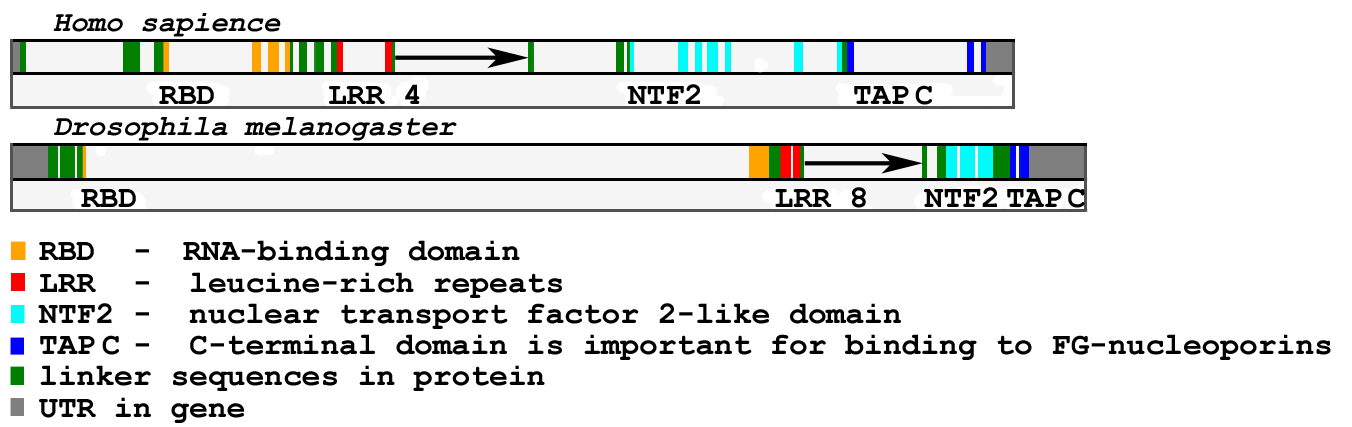
\includegraphics[width=0.9\textwidth]{images/dm_hs_nxf1_structure}
%    \caption{Интрон-экзонная структура для генов \textit{Hs Nxf1} и \textit{Dm Nxf1}. Стрелки обозначают ``кассетный`` интрон. Цвета экзонов отображают белковые домены~\cite{Mamon2013}.}
%    \label{fig:dm_hs_nxf1_structure}
%\end{figure}
%
%Основной и общеизвестной функцией продукта гена \textit{Nxf1} является транспорт всех типов мРНК из ядра в цитоплазму~\cite{Herold2000}.
%Кассетный интрон условно разделяет \textit{Nxf1} на две функциональные половины – рецепторную, куда относятся RBD и LRR, отвечающую за взаимодействие с РНК, и транспортную, куда входят NTF2L и UBA, позволяющую, взаимодействуя с другими белками, обеспечивать транспорт комплекса макромолекул через ядерные поры~\cite{Mamon2013}.
%
%Помимо классической функции нашей группой выявлены дополнительные, жизненно важные функции продукта гена \textit{Nxf1}, или \textit{sbr} у дрозофилид.
%Во-первых, доказано, что sbr выполняет семенниково-специфические функции.
%Показано, что существуют специфичные для семенников альтернативные транскрипты, полученные за счет альтернативного промотора, этого гена и укороченный белок sbr, обнаруженный только в семенниках~\cite{Ginanova2016}.
%
%Во-вторых, установлено, что белок sbr необходим для формирования внутренней структуры и установления границ в мозговом веществе зрительной системы дрозофилы.
%Распределение sbr в ядре и цитоплазме специфических нейронов и глиальных клеток свидетельствует о специализированных функциях этого белка~\cite{Mamon2021}.
%
%Также в одной из недавних работ была продемонстрирована значимость ``кассетного`` интрона в эволюции гена \textit{Nxf1} у представителей Chiroptera~\cite{Bondaruk2022}.
%
%В моей бакалаврской работе было проанализировано 89 нуклеотидных последовательностей гена \textit{Nxf1} из таксономической группы Arthropoda, а также найдены последовательности гена для 37 представителей дрозофилид.
%По результатам проведенных множественных выравниваний и построенных вторичных структур интрон-содержащего транскрипта были сформулированы следующие выводы:
%
%\begin{enumerate}[left=\parindent]
%    \item Структура ``консервативной кассеты`` является специфической для таксонов низкого ранга у всех взятых в анализ артропод.
%    \item Интрон-содержащие транскрипты формируют специфические вторичные структуры; у дрозофилид продемонстрировано наличие А-обогащенных участков.
%\end{enumerate}
%
%Таким образом, важность роли гена \textit{Nxf1} и ``кассетного`` интрона в нем не вызывает сомнений.
%Тем не менее очень интересно было бы проанализировать структуру данного гена у представителей за пределами Arthropoda, используя современные методы биоинформатики, освоенные в магистратуре, о чем и пойдет речь далее.


% Материалы и методы
\newpage
\section{Материалы и методы}

\subsection{Первичный анализ}

В качестве отправной точки был произведен поиск гена \textit{Nxf1} внутри веб-сервиса NCBI~\cite{ncbi_general}.
Полученные данные были сохранены в текстовом формате и загружены в виде tsv-таблицы с помощью пакета pandas v2.2.3~\cite{pandas} для языка программирования Python v3.12.6~\cite{python_3_12}.
Всего был найден 651 вид, содержащий анализируемый ген, большинство из которых относятся к Deuterostomia (Вторичноротые) – 436 видов.
Таким образом, в качестве материалов выступали нуклеотидные и белковые последовательности, соответствующие гену \textit{Nxf1}, из открытых баз данных NCBI~\cite{ncbi_general}.

Большинство этапов последующего анализа реализовано в виде отдельных скриптов, разработанных в рамках данной работы, если не указано другое.
Для логического разделения на блоки был использован Jupyter Notebook v1.1.1~\cite{jupyter_notebook}.

По данным из полученной таблицы в порядке поискового эксперимента было построено филогенетическое дерево по найденным видам для оценки количества видов в таксонах более низкого ранга.
Для глубокого анализа было принято решение сфокусироваться на организмах, относящихся к группе Protostomia (Первичноротые), Cnidaria (Стрекающие), а также на всех группах из Deuterostomia за исключением Mammalia (Млекопитающие).

\subsection{Загрузка данных}

Для найденных организмов с помощью пакета NCBI E-utilities из BioPython v1.85~\cite{biopython} и NCBI Datasets Command-Line Interface (CLI) v18.0.2~\cite{datasets} были загружены нуклеотидные последовательности гена, кодирующих участков и мРНК, а также аминокислотные последовательности белка в формате FASTA и аннотации для гена в GenBank-формате, необходимые для получения нуклеотидных последовательностей экзонов и поиска ``консервативной кассеты``.
Затем были получены и проанализированы интересующие нас участки экзон-интрон-экзонной структуры и созданы файлы со всеми экзонами и ``кассетным`` интроном для всех организмов, у которых получилось найти ``кассету``.
Данные файлы будут необходимы для последующего анализа.

\subsection{Увеличение выборок}

Учитывая очень маленькие выборки во многих анализируемых группах (например, Cnidaria – 4 вида, Spiralia – 9 видов), было принято решение по увеличению их количества.
Для этой цели, учитывая разнообразия полученных генов даже внутри одной таксономической группы, самым эффективным вариантом оказалось использование PSI-BLAST~\cite{psi_blast}.
В качестве запроса (Query), или референса, использовались белковые последовательности тех организмов, у которых была найдена ``кассета``.
Для проведения PSI-BLAST были выбраны настройки по-умолчанию за исключением параметра Organism: поиск проводился внутри таксономической группы, к которой принадлежал референс, также референс был исключен из поиска.

\subsection{Парсинг результатов}

Парсинг результатов BLAST также осуществлялся с помощью пакета BioPython~\cite{biopython} и специально разработанных скриптов.
Он включал в себя фильтрацию данных по параметрам процента покрытия (Query Coverage, QC), длине и сходству (Per. Ident) найденных последовательностей (Subject), а также загрузку нуклеотидных и белковых последовательностей, однако реализация отличалась из-за особенностей баз данных NCBI~\cite{ncbi_general}.
Получение ``кассеты`` было произведено по тому же принципу, но, опять же, с отличиями.
Благодаря данному шагу удалось увеличить выборки суммарно на 117 видов.
К сожалению, для некоторых таксономических групп увеличение выборки оказалось невозможным в связи с отсутствием у некоторых организмов интересующего нас участка.

\subsection{Множественные выравнивания}

Множественные выравнивания осуществлялись с помощью алгоритма MAFFT~\cite{mafft}, 10 итераций, остальные настройки по-умолчанию, в программе Unipro UGENE v52.0~\cite{ugene}.

\subsection{Поиск консервативных мотивов внутри ``кассетного`` интрона}

Анализ видов из Deuterostomia изначально шел более благоприятно за счет большого сходства последовательностей, в том числе интронных, и большего количества видов в группах.
Для них также были загружены все необходимые файлы и произведен поиск и анализ ``консервативной кассеты``.
Мы решили сосредоточить свое внимание на организмах из Actinopterygii (Лучеперые рыбы), 72 вида, так как данных по ним ранее получено не было.

Учитывая большую степень сходства интронных последовательностей, с помощью пакета инструментов MEME Suite v5.5.8~\cite{meme} локально был произведен поиск консервативных мотивов внутри ``кассетного`` интрона.
Найденные мотивы, у которых E-value < 0.05 также локально были проанализированы с помощью Tomtom~\cite{tomtom} из того же пакета.
Для описанного шага была взята база данных JASPAR2024 CORE (NON-REDUNDANT) DNA.

\subsection{Построение и анализ вторичных структур РНК}

С помощью инструмента RNAfold v2.7.0 из пакета Vienna\-RNA~\cite{viennarna} были построены вторичные структуры РНК для нуклеотидных последовательностей в двух вариантах (MFE и Centroid), содержащих экзоны и ``кассетный`` интрон, так как мы предполагаем, что избегание интроном сплайсинга может быть опосредовано образованной им специфической вторичной структурой.
Учитывая данное предположение, разумным шагом также являлся анализ ``силы сайтов сплайсинга``, проведенный с помощью MaxEntScan~\cite{maxentsccan}.
Также с помощью скриптов цветом были выделены интронные последовательности внутри вторичной структуры и найденный мотив у Actinopterygii, который предположительно является CTE (Constitutive Transport Element).

\subsection{Филогенетический анализ}

Для Actinopterygii также был проведен филогенетический анализ, включающий построение и визуализацию деревьев.
Для данной цели использовались самые популярные и проверенные временем инструменты.
Построение деревьев осуществлялось с помощью IQ-TREE v2.4.0~\cite{iqtree2}, визуализация – с помощью Figtree v1.4.4~\cite{figtree}.

\subsection{Настройки системы и доступность скриптов}

Работа проводилась в виртуальном окружении Mamba v1.5.5~\cite{mamba}, использованные пакеты и примеры анализа в Jupyter Notebooks можно найти в GitHub~\cite{github_general} репозитории автора: \url{https://github.com/ArtemVaska/Diploma}.

Для написания ВКР была использована система верстки LaTeX v4.76~\cite{latex}, таблицы генерировались в веб-сервисе TablesGenerator~\cite{tablesgenerator}.
Большинство картинок создано с помощью веб-сервиса draw.io~\cite{drawio}.

Все шаги анализа проводились на базе операционной системы Linux Ubuntu 22.04~\cite{ubuntu}.


% Результаты и обсуждение
\newpage
\section{Результаты и обсуждение}

Текст...


% Выводы
% \clearpage
\section{Выводы}

\begin{enumerate}[left=\parindent]
    \item Внутри одной таксономической группы существуют преобладающие значения для характеристик ``консервативной кассеты``:
    \begin{itemize}
        \item длина первого и второго экзона;
        \item длина ``кассетного`` интрона;
        \item длина участка внутри ``кассетного`` интрона до стоп-кодона.
    \end{itemize}
    \item Внутри ``кассетного`` интрона существуют участки, которые образуют особые структуры при формировании вторичной структуры интрон-содержащего транскрипта, и за счет их наличия возможно сохранение такого транскрипта и последующая трансляция с синтезом укороченной формы белка.
\end{enumerate}


% Таблицы с результатами (временный раздел)
\newpage
\section{Таблицы с результатами}

\begin{longtable}[c]{|c|c|c|c|c|}
\caption{Сводная таблица с характеристикой кассетного интрона для таксономической группы Actinopterygii.
Сортировка по возрастанию количества нуклеотидов до стоп-кодона в кассетной интроне.}
\label{tab:Actinopterygii}\\
\hline
\textbf{\begin{tabular}[c]{@{}c@{}}Название\\ организма\end{tabular}} &
  \textbf{\begin{tabular}[c]{@{}c@{}}Кол-во\\ нуклеотидов\\ до стоп-кодона\\ в интроне\end{tabular}} &
  \textbf{\begin{tabular}[c]{@{}c@{}}Длина\\ 1-го экзона\\ в кассете\end{tabular}} &
  \textbf{\begin{tabular}[c]{@{}c@{}}Длина\\ кассетного\\ интрона\end{tabular}} &
  \textbf{\begin{tabular}[c]{@{}c@{}}Длина\\ 2-го экзона\\ в кассете\end{tabular}} \\ \hline
\endfirsthead
%
\endhead
%
\hline
\endfoot
%
\endlastfoot
%
\textit{Chanos chanos}                 & 1   & 110 & 3568 & 37 \\
\textit{Danio rerio}                   & 1   & 110 & 3580 & 37 \\
\textit{Denticeps clupeoides}          & 7   & 110 & 2629 & 37 \\
\textit{Labrus bergylta}               & 10  & 110 & 2684 & 37 \\
\textit{Cottoperca gobio}              & 16  & 110 & 2388 & 37 \\
\textit{Xiphophorus couchianus}        & 22  & 110 & 2227 & 37 \\
\textit{Larimichthys crocea}           & 22  & 110 & 2340 & 37 \\
\textit{Lates calcarifer}              & 22  & 110 & 2434 & 37 \\
\textit{Notothenia coriiceps}          & 22  & 110 & 2886 & 37 \\
\textit{Betta splendens}               & 22  & 110 & 2274 & 37 \\
\textit{Poecilia reticulata}           & 22  & 110 & 2262 & 37 \\
\textit{Takifugu rubripes}             & 22  & 110 & 2114 & 37 \\
\textit{Salarias fasciatus}            & 22  & 110 & 3855 & 37 \\
\textit{Poecilia mexicana}             & 22  & 110 & 2247 & 37 \\
\textit{Stegastes partitus}            & 22  & 110 & 2900 & 37 \\
\textit{Clupea harengus}               & 22  & 110 & 3219 & 37 \\
\textit{Archocentrus centrarchus}      & 22  & 110 & 2644 & 37 \\
\textit{Esox lucius}                   & 22  & 110 & 2848 & 37 \\
\textit{Monopterus albus}              & 22  & 110 & 2353 & 37 \\
\textit{Echeneis naucrates}            & 22  & 110 & 2314 & 37 \\
\textit{Paralichthys olivaceus}        & 22  & 110 & 3148 & 37 \\
\textit{Maylandia zebra}               & 22  & 110 & 2565 & 37 \\
\textit{Parambassis ranga}             & 22  & 110 & 2484 & 37 \\
\textit{Sander lucioperca}             & 22  & 110 & 2494 & 37 \\
\textit{Xiphophorus maculatus}         & 22  & 110 & 2231 & 37 \\
\textit{Nothobranchius furzeri}        & 22  & 110 & 2290 & 37 \\
\textit{Anabas testudineus}            & 22  & 110 & 2352 & 37 \\
\textit{Acanthochromis polyacanthus}   & 22  & 110 & 2797 & 37 \\
\textit{Anarrhichthys ocellatus}       & 22  & 110 & 2355 & 37 \\
\textit{Boleophthalmus pectinirostris} & 22  & 110 & 1702 & 37 \\
\textit{Sparus aurata}                 & 22  & 110 & 2361 & 37 \\
\textit{Oryzias melastigma}            & 22  & 110 & 2212 & 37 \\
\textit{Seriola dumerili}              & 22  & 110 & 2494 & 37 \\
\textit{Poecilia formosa}              & 22  & 110 & 2259 & 37 \\
\textit{Oreochromis niloticus}         & 22  & 110 & 2580 & 37 \\
\textit{Kryptolebias marmoratus}       & 22  & 110 & 2556 & 37 \\
\textit{Xiphophorus hellerii}          & 22  & 110 & 2240 & 37 \\
\textit{Poecilia latipinna}            & 22  & 110 & 2261 & 37 \\
\textit{Pundamilia nyererei}           & 22  & 110 & 2527 & 37 \\
\textit{Hippocampus comes}             & 22  & 110 & 2622 & 37 \\
\textit{Oreochromis aureus}            & 22  & 110 & 2579 & 37 \\
\textit{Amphiprion ocellaris}          & 22  & 110 & 2752 & 37 \\
\textit{Seriola lalandi dorsalis}      & 22  & 110 & 2481 & 37 \\
\textit{Austrofundulus limnaeus}       & 22  & 110 & 2541 & 37 \\
\textit{Puntigrus tetrazona}           & 25  & 110 & 2440 & 37 \\
\textit{Fundulus heteroclitus}         & 25  & 110 & 2476 & 37 \\
\textit{Cyprinodon variegatus}         & 28  & 110 & 2533 & 37 \\
\textit{Haplochromis burtoni}          & 31  & 110 & 2535 & 37 \\
\textit{Astatotilapia calliptera}      & 31  & 110 & 2571 & 37 \\
\textit{Gouania willdenowi}            & 37  & 110 & 2616 & 37 \\
\textit{Oryzias latipes}               & 40  & 110 & 2331 & 37 \\
\textit{Sphaeramia orbicularis}        & 43  & 110 & 2376 & 37 \\
\textit{Pygocentrus nattereri}         & 46  & 110 & 2649 & 37 \\
\textit{Astyanax mexicanus}            & 46  & 110 & 2791 & 37 \\
\textit{Colossoma macropomum}          & 46  & 110 & 2644 & 37 \\
\textit{Ictalurus punctatus}           & 46  & 110 & 3166 & 37 \\
\textit{Tachysurus fulvidraco}         & 46  & 110 & 3493 & 37 \\
\textit{Pangasianodon hypophthalmus}   & 46  & 110 & 3348 & 37 \\
\textit{Erpetoichthys calabaricus}     & 55  & 110 & 3662 & 37 \\
\textit{Perca flavescens}              & 58  & 110 & 2378 & 37 \\
\textit{Mastacembelus armatus}         & 64  & 110 & 2371 & 37 \\
\textit{Salmo salar}                   & 67  & 110 & 3553 & 37 \\
\textit{Gadus morhua}                  & 67  & 110 & 3151 & 37 \\
\textit{Etheostoma spectabile}         & 97  & 110 & 2457 & 37 \\
\textit{Scleropages formosus}          & 112 & 110 & 3412 & 37 \\
\textit{Myripristis murdjan}           & 112 & 110 & 2492 & 37 \\
\textit{Paramormyrops kingsleyae}      & 121 & 110 & 2929 & 37 \\
\textit{Carassius auratus}             & 148 & 110 & 3854 & 37 \\
\textit{Sinocyclocheilus grahami}      & 148 & 110 & 3330 & 37 \\
\textit{Sinocyclocheilus rhinocerous}  & 154 & 110 & 3449 & 37 \\
\textit{Sinocyclocheilus anshuiensis}  & 154 & 110 & 4202 & 37 \\
\textit{Electrophorus electricus}      & 283 & 110 & 2874 & 37 \\ \hline
\end{longtable}


\begin{longtable}[c]{|c|c|c|c|c|}
\caption{Сводная таблица с характеристикой кассетного интрона для таксономической группы Amphibia.
Сортировка по возрастанию количества нуклеотидов до стоп-кодона в кассетной интроне.}
\label{tab:Amphibia}\\
\hline
\textbf{\begin{tabular}[c]{@{}c@{}}Название\\ организма\end{tabular}} &
  \textbf{\begin{tabular}[c]{@{}c@{}}Кол-во\\ нуклеотидов\\ до стоп-кодона\\ в интроне\end{tabular}} &
  \textbf{\begin{tabular}[c]{@{}c@{}}Длина\\ 1-го экзона\\ в кассете\end{tabular}} &
  \textbf{\begin{tabular}[c]{@{}c@{}}Длина\\ кассетного\\ интрона\end{tabular}} &
  \textbf{\begin{tabular}[c]{@{}c@{}}Длина\\ 2-го экзона\\ в кассете\end{tabular}} \\ \hline
\endfirsthead
%
\endhead
%
\hline
\endfoot
%
\endlastfoot
%
Ambystoma mexicanum     & 1   & 110 & 10340 & 37 \\
Pelobates fuscus        & 1   & 110 & 2424  & 37 \\
Bufo bufo               & 7   & 110 & 3002  & 37 \\
Bufo gargarizans        & 7   & 110 & 2879  & 37 \\
Hyperolius riggenbachi  & 10  & 110 & 3902  & 37 \\
Rana temporaria         & 10  & 110 & 3036  & 37 \\
Pseudophryne corroboree & 19  & 110 & 3561  & 37 \\
Spea bombifrons         & 25  & 110 & 2840  & 37 \\
Engystomops pustulosus  & 25  & 110 & 2004  & 37 \\
Nanorana parkeri        & 25  & 110 & 3038  & 37 \\
Hyla sarda              & 25  & 110 & 3029  & 37 \\
Pyxicephalus adspersus  & 25  & 110 & 2917  & 37 \\
Ranitomeya imitator     & 37  & 110 & 2650  & 37 \\
Xenopus tropicalis      & 46  & 110 & 2596  & 37 \\
Xenopus laevis          & 52  & 110 & 3791  & 37 \\
Geotrypetes seraphini   & 55  & 110 & 3065  & 37 \\
Rhinatrema bivittatum   & 103 & 110 & 4053  & 37 \\
Pleurodeles waltl       & 151 & 110 & 3245  & 37 \\
Microcaecilia unicolor  & 187 & 110 & 2784  & 37 \\ \hline
\end{longtable}


% Please add the following required packages to your document preamble:
% \usepackage{longtable}
% Note: It may be necessary to compile the document several times to get a multi-page table to line up properly
\begin{longtable}[c]{|c|c|c|c|c|}
\caption{Сводная таблица с характеристикой кассетного интрона для таксономической группы Cnidaria.
Сортировка по возрастанию количества нуклеотидов до стоп-кодона в кассетной интроне.}
\label{tab:Cnidaria}\\
\hline
\textbf{\begin{tabular}[c]{@{}c@{}}Название\\ организма\end{tabular}} &
  \textbf{\begin{tabular}[c]{@{}c@{}}Кол-во\\ нуклеотидов\\ до стоп-кодона\\ в интроне\end{tabular}} &
  \textbf{\begin{tabular}[c]{@{}c@{}}Длина\\ 1-го экзона\\ в кассете\end{tabular}} &
  \textbf{\begin{tabular}[c]{@{}c@{}}Длина\\ кассетного\\ интрона\end{tabular}} &
  \textbf{\begin{tabular}[c]{@{}c@{}}Длина\\ 2-го экзона\\ в кассете\end{tabular}} \\ \hline
\endfirsthead
%
\endhead
%
\hline
\endfoot
%
\endlastfoot
%
\textit{Actinia tenebrosa}       & 10  & 116 & 173 & 37 \\
\textit{Dendronephthya gigantea} & 10  & 116 & 328 & 37 \\
\textit{Nematostella vectensis}  & 25  & 116 & 991 & 37 \\
\textit{Montipora foliosa}       & 31  & 116 & 907 & 37 \\
\textit{Pocillopora verrucosa}   & 34  & 116 & 390 & 37 \\
\textit{Acropora digitifera}     & 40  & 116 & 670 & 37 \\
\textit{Acropora millepora}      & 40  & 116 & 682 & 37 \\
\textit{Acropora muricata}       & 40  & 116 & 679 & 37 \\
\textit{Pocillopora damicornis}  & 46  & 116 & 392 & 37 \\
\textit{Pocillopora meandrina}   & 46  & 116 & 392 & 37 \\
\textit{Porites lutea}           & 61  & 116 & 711 & 37 \\
\textit{Porites evermanni}       & 61  & 116 & 711 & 37 \\
\textit{Exaiptasia diaphana}     & 76  & 86  & 227 & 37 \\
\textit{Xenia sp. Carnegie-2017} & 103 & 116 & 116 & 37 \\ \hline
\end{longtable}


% Please add the following required packages to your document preamble:
% \usepackage{longtable}
% Note: It may be necessary to compile the document several times to get a multi-page table to line up properly
\begin{longtable}[c]{|c|c|c|c|c|}
\caption{Сводная таблица с характеристикой кассетного интрона для таксономической группы Ecdysozoa.
Сортировка по возрастанию количества нуклеотидов до стоп-кодона в кассетной интроне.}
\label{tab:Ecdysozoa}\\
\hline
\textbf{\begin{tabular}[c]{@{}c@{}}Название\\ организма\end{tabular}} &
  \textbf{\begin{tabular}[c]{@{}c@{}}Кол-во\\ нуклеотидов\\ до стоп-кодона\\ в интроне\end{tabular}} &
  \textbf{\begin{tabular}[c]{@{}c@{}}Длина\\ 1-го экзона\\ в кассете\end{tabular}} &
  \textbf{\begin{tabular}[c]{@{}c@{}}Длина\\ кассетного\\ интрона\end{tabular}} &
  \textbf{\begin{tabular}[c]{@{}c@{}}Длина\\ 2-го экзона\\ в кассете\end{tabular}} \\ \hline
\endfirsthead
%
\endhead
%
\hline
\endfoot
%
\endlastfoot
%
\textit{Trichinella spiralis}             & 1    & 83  & 417  & 37 \\
\textit{Priapulus caudatus}               & 1    & 110 & 2114 & 37 \\
\textit{Galendromus occidentalis}         & 1    & 110 & 1491 & 37 \\
\textit{Ixodes scapularis}                & 1    & 110 & 3567 & 37 \\
\textit{Limulus polyphemus}               & 1    & 110 & 915  & 37 \\
\textit{Parasteatoda tepidariorum}        & 1    & 110 & 1725 & 37 \\
\textit{Cryptotermes secundus}            & 1    & 110 & 4335 & 37 \\
\textit{Maniola hyperantus}               & 1    & 110 & 920  & 37 \\
\textit{Cimex lectularius}                & 1    & 110 & 4437 & 37 \\
\textit{Vespa mandarinia}                 & 1    & 113 & 379  & 37 \\
\textit{Zerene cesonia}                   & 1    & 110 & 1162 & 37 \\
\textit{Pararge aegeria}                  & 1    & 110 & 2657 & 37 \\
\textit{Myzus persicae}                   & 1    & 107 & 772  & 37 \\
\textit{Halyomorpha halys}                & 1    & 110 & 7270 & 37 \\
\textit{Diuraphis noxia}                  & 1    & 107 & 742  & 37 \\
\textit{Sipha flava}                      & 1    & 107 & 58   & 37 \\
\textit{Manduca sexta}                    & 1    & 110 & 1796 & 37 \\
\textit{Apis laboriosa}                   & 1    & 113 & 1254 & 37 \\
\textit{Orussus abietinus}                & 1    & 113 & 74   & 37 \\
\textit{Danaus plexippus}                 & 1    & 110 & 1009 & 37 \\
\textit{Colletes gigas}                   & 1    & 113 & 379  & 37 \\
\textit{Ostrinia furnacalis}              & 1    & 110 & 1946 & 37 \\
\textit{Vespa crabro}                     & 1    & 113 & 381  & 37 \\
\textit{Venturia canescens}               & 1    & 113 & 621  & 37 \\
\textit{Papilio polytes}                  & 1    & 110 & 1674 & 37 \\
\textit{Vespa velutina}                   & 1    & 113 & 377  & 37 \\
\textit{Cephus cinctus}                   & 1    & 113 & 75   & 37 \\
\textit{Bombus pyrosoma}                  & 1    & 113 & 244  & 37 \\
\textit{Papilio xuthus}                   & 1    & 110 & 999  & 37 \\
\textit{Vanessa tameamea}                 & 1    & 110 & 2352 & 37 \\
\textit{Megalopta genalis}                & 1    & 113 & 373  & 37 \\
\textit{Vespula pensylvanica}             & 1    & 113 & 363  & 37 \\
\textit{Leptopilina heterotoma}           & 1    & 113 & 921  & 37 \\
\textit{Acromyrmex echinatior}            & 1    & 113 & 438  & 37 \\
\textit{Aphidius gifuensis}               & 1    & 113 & 240  & 37 \\
\textit{Polistes fuscatus}                & 1    & 113 & 400  & 37 \\
\textit{Dirofilaria immitis}              & 7    & 98  & 248  & 37 \\
\textit{Odontomachus brunneus}            & 10   & 113 & 498  & 37 \\
\textit{Diploscapter pachys}              & 10   & 110 & 662  & 37 \\
\textit{Bactrocera dorsalis}              & 13   & 110 & 1808 & 37 \\
\textit{Drosophila melanogaster}          & 13   & 110 & 1602 & 37 \\
\textit{Ceratitis capitata}               & 19   & 110 & 2023 & 37 \\
\textit{Pediculus humanus corporis}       & 19   & 110 & 631  & 37 \\
\textit{Aphelenchoides avenae}            & 19   & 110 & 441  & 37 \\
\textit{Litomosoides sigmodontis}         & 19   & 110 & 242  & 37 \\
\textit{Acanthocheilonema viteae}         & 19   & 110 & 225  & 37 \\
\textit{Aethina tumida}                   & 19   & 110 & 1729 & 37 \\
\textit{Lepeophtheirus salmonis}          & 22   & 110 & 1555 & 37 \\
\textit{Anoplophora glabripennis}         & 22   & 110 & 3664 & 37 \\
\textit{Varroa jacobsoni}                 & 22   & 110 & 3077 & 37 \\
\textit{Varroa destructor}                & 22   & 110 & 3077 & 37 \\
\textit{Thelazia callipaeda}              & 25   & 110 & 209  & 37 \\
\textit{Bursaphelenchus xylophilus}       & 25   & 110 & 638  & 37 \\
\textit{Acyrthosiphon pisum}              & 28   & 107 & 68   & 37 \\
\textit{Anisakis simplex}                 & 30   & 219 & 665  & 37 \\
\textit{Tetranychus urticae}              & 31   & 122 & 648  & 37 \\
\textit{Homarus americanus}               & 31   & 110 & 9821 & 37 \\
\textit{Bursaphelenchus okinawaensis}     & 37   & 110 & 593  & 37 \\
\textit{Globodera pallida}                & 43   & 113 & 47   & 37 \\
\textit{Amphibalanus amphitrite}          & 73   & 110 & 369  & 37 \\
\textit{Cotesia glomerata}                & 73   & 116 & 236  & 37 \\
\textit{Caenorhabditis angaria}           & 79   & 110 & 96   & 37 \\
\textit{Onchocerca ochengi}               & 88   & 110 & 243  & 37 \\
\textit{Brugia pahangi}                   & 91   & 110 & 232  & 37 \\
\textit{Ditylenchus destructor}           & 97   & 307 & 1167 & 37 \\
\textit{Mesorhabditis belari}             & 97   & 110 & 147  & 37 \\
\textit{Melanaphis sacchari}              & 97   & 107 & 71   & 37 \\
\textit{Enterobius vermicularis}          & 100  & 110 & 195  & 37 \\
\textit{Pristionchus mayeri}              & 103  & 110 & 131  & 37 \\
\textit{Cercopithifilaria johnstoni}      & 103  & 110 & 238  & 37 \\
\textit{Steinernema carpocapsae}          & 106  & 110 & 131  & 37 \\
\textit{Wuchereria bancrofti}             & 106  & 125 & 242  & 37 \\
\textit{Parelaphostrongylus tenuis}       & 112  & 110 & 228  & 37 \\
\textit{Toxocara canis}                   & 115  & 110 & 1062 & 37 \\
\textit{Necator americanus}               & 136  & 110 & 243  & 37 \\
\textit{Brugia malayi}                    & 139  & 110 & 243  & 37 \\
\textit{Caenorhabditis auriculariae}      & 145  & 110 & 156  & 37 \\
\textit{Auanema sp. JU1783}               & 145  & 110 & 80   & 37 \\
\textit{Pristionchus entomophagus}        & 151  & 110 & 154  & 37 \\
\textit{Steinernema hermaphroditum}       & 157  & 110 & 131  & 37 \\
\textit{Caenorhabditis brenneri}          & 175  & 110 & 130  & 37 \\
\textit{Angiostrongylus cantonensis}      & 181  & 110 & 213  & 37 \\
\textit{Dictyocaulus viviparus}           & 190  & 110 & 832  & 37 \\
\textit{Caenorhabditis elegans}           & 193  & 110 & 106  & 37 \\
\textit{Cooperia oncophora}               & 205  & 110 & 215  & 37 \\
\textit{Caenorhabditis sp. 36 PRJEB53466} & 205  & 110 & 133  & 37 \\
\textit{Caenorhabditis nigoni}            & 214  & 110 & 142  & 37 \\
\textit{Pristionchus pacificus}           & 214  & 110 & 251  & 37 \\
\textit{Trichostrongylus colubriformis}   & 214  & 110 & 224  & 37 \\
\textit{Caenorhabditis briggsae}          & 217  & 110 & 145  & 37 \\
\textit{Cylicocyclus nassatus}            & 229  & 110 & 239  & 37 \\
\textit{Haemonchus contortus}             & 304  & 110 & 220  & 37 \\
\textit{Caenorhabditis bovis}             & 316  & 110 & 235  & 37 \\
\textit{Nippostrongylus brasiliensis}     & 316  & 110 & 235  & 37 \\
\textit{Dracunculus medinensis}           & 334  & 110 & 122  & 37 \\
\textit{Mesorhabditis spiculigera}        & 376  & 110 & 173  & 37 \\
\textit{Pollicipes pollicipes}            & 436  & 110 & 367  & 37 \\
\textit{Rhopalosiphum maidis}             & 1345 & 107 & 69   & 37 \\ \hline
\end{longtable}


% Please add the following required packages to your document preamble:
% \usepackage{longtable}
% Note: It may be necessary to compile the document several times to get a multi-page table to line up properly
\begin{longtable}[c]{|c|c|c|c|c|}
\caption{Сводная таблица с характеристикой кассетного интрона для таксономической группы Lepidosauria.
Сортировка по возрастанию количества нуклеотидов до стоп-кодона в кассетной интроне.}
\label{tab:Lepidosauria}\\
\hline
\textbf{\begin{tabular}[c]{@{}c@{}}Название\\ организма\end{tabular}} &
  \textbf{\begin{tabular}[c]{@{}c@{}}Кол-во\\ нуклеотидов\\ до стоп-кодона\\ в интроне\end{tabular}} &
  \textbf{\begin{tabular}[c]{@{}c@{}}Длина\\ 1-го экзона\\ в кассете\end{tabular}} &
  \textbf{\begin{tabular}[c]{@{}c@{}}Длина\\ кассетного\\ интрона\end{tabular}} &
  \textbf{\begin{tabular}[c]{@{}c@{}}Длина\\ 2-го экзона\\ в кассете\end{tabular}} \\ \hline
\endfirsthead
%
\endhead
%
\hline
\endfoot
%
\endlastfoot
%
\textit{Python bivittatus}             & 1 & 110 & 2374 & 37 \\
\textit{Notechis scutatus}             & 1 & 110 & 2507 & 37 \\
\textit{Pseudonaja textilis}           & 1 & 110 & 2519 & 37 \\
\textit{Anolis sagrei}                 & 1 & 110 & 4667 & 37 \\
\textit{Pituophis catenifer annectens} & 1 & 110 & 2420 & 37 \\
\textit{Lacerta agilis}                & 1 & 110 & 2499 & 37 \\
\textit{Candoia aspera}                & 1 & 110 & 2293 & 37 \\
\textit{Sphaerodactylus townsendi}     & 1 & 110 & 2825 & 37 \\
\textit{Thamnophis elegans}            & 1 & 110 & 2426 & 37 \\
\textit{Ahaetulla prasina}             & 1 & 110 & 2432 & 37 \\
\textit{Gekko japonicus}               & 1 & 110 & 2924 & 37 \\
\textit{Crotalus tigris}               & 1 & 110 & 3091 & 37 \\
\textit{Pogona vitticeps}              & 1 & 110 & 2746 & 37 \\
\textit{Podarcis raffonei}             & 1 & 110 & 2495 & 37 \\
\textit{Protobothrops mucrosquamatus}  & 1 & 110 & 3264 & 37 \\
\textit{Varanus komodoensis}           & 1 & 110 & 2658 & 37 \\
\textit{Pantherophis guttatus}         & 1 & 110 & 2411 & 37 \\
\textit{Elgaria multicarinata webbii}  & 1 & 110 & 2800 & 37 \\
\textit{Rhineura floridana}            & 1 & 110 & 2581 & 37 \\
\textit{Podarcis muralis}              & 1 & 110 & 2506 & 37 \\
\textit{Heteronotia binoei}            & 1 & 110 & 3002 & 37 \\
\textit{Anolis carolinensis}           & 1 & 110 & 4026 & 37 \\
\textit{Erythrolamprus reginae}        & 1 & 110 & 2638 & 37 \\
\textit{Sceloporus undulatus}          & 1 & 110 & 2380 & 37 \\
\textit{Eublepharis macularius}        & 1 & 110 & 2577 & 37 \\
\textit{Euleptes europaea}             & 1 & 110 & 2901 & 37 \\
\textit{Hemicordylus capensis}         & 1 & 110 & 2830 & 37 \\
\textit{Zootoca vivipara}              & 1 & 110 & 2516 & 37 \\ \hline
\end{longtable}


% Please add the following required packages to your document preamble:
% \usepackage{longtable}
% Note: It may be necessary to compile the document several times to get a multi-page table to line up properly
\begin{longtable}[c]{|c|c|c|c|c|}
\caption{Сводная таблица с характеристикой кассетного интрона для таксономической группы Sauropsida.
Сортировка по возрастанию количества нуклеотидов до стоп-кодона в кассетной интроне.}
\label{tab:Sauropsida}\\
\hline
\textbf{\begin{tabular}[c]{@{}c@{}}Название\\ организма\end{tabular}} &
  \textbf{\begin{tabular}[c]{@{}c@{}}Кол-во\\ нуклеотидов\\ до стоп-кодона\\ в интроне\end{tabular}} &
  \textbf{\begin{tabular}[c]{@{}c@{}}Длина\\ 1-го экзона\\ в кассете\end{tabular}} &
  \textbf{\begin{tabular}[c]{@{}c@{}}Длина\\ кассетного\\ интрона\end{tabular}} &
  \textbf{\begin{tabular}[c]{@{}c@{}}Длина\\ 2-го экзона\\ в кассете\end{tabular}} \\ \hline
\endfirsthead
%
\endhead
%
\hline
\endfoot
%
\endlastfoot
%
\textit{Molothrus aeneus}             & 1    & 110 & 745  & 37 \\
\textit{Taeniopygia guttata}          & 1    & 110 & 443  & 37 \\
\textit{Lonchura striata}             & 1    & 110 & 629  & 37 \\
\textit{Gallus gallus}                & 7    & 110 & 1616 & 37 \\
\textit{Cygnus atratus}               & 25   & 110 & 1257 & 37 \\
\textit{Haliaeetus leucocephalus}     & 25   & 110 & 1375 & 37 \\
\textit{Phalacrocorax carbo}          & 25   & 110 & 1345 & 37 \\
\textit{Grus americana}               & 25   & 110 & 1659 & 37 \\
\textit{Haliaeetus albicilla}         & 25   & 110 & 1378 & 37 \\
\textit{Oxyura jamaicensis}           & 25   & 110 & 1246 & 37 \\
\textit{Anser cygnoides}              & 25   & 110 & 1279 & 37 \\
\textit{Ciconia boyciana}             & 25   & 107 & 1459 & 37 \\
\textit{Anas acuta}                   & 25   & 110 & 1346 & 37 \\
\textit{Astur gentilis}               & 25   & 110 & 1393 & 37 \\
\textit{Aquila chrysaetos chrysaetos} & 25   & 110 & 1375 & 37 \\
\textit{Aythya fuligula}              & 25   & 110 & 1227 & 37 \\
\textit{Struthio camelus}             & 64   & 110 & 1405 & 37 \\
\textit{Chelonia mydas}               & 79   & 110 & 1674 & 37 \\
\textit{Dermochelys coriacea}         & 79   & 110 & 1661 & 37 \\
\textit{Caretta caretta}              & 79   & 110 & 1656 & 37 \\
\textit{Ammospiza caudacuta}          & 82   & 110 & 3942 & 37 \\
\textit{Aphelocoma coerulescens}      & 85   & 110 & 3626 & 37 \\
\textit{Gopherus flavomarginatus}     & 142  & 110 & 1655 & 37 \\
\textit{Chelonoidis abingdonii}       & 142  & 110 & 1645 & 37 \\
\textit{Malaclemys terrapin pileata}  & 142  & 110 & 1652 & 37 \\
\textit{Mauremys mutica}              & 142  & 110 & 1662 & 37 \\
\textit{Mauremys reevesii}            & 142  & 110 & 1661 & 37 \\
\textit{Trachemys scripta elegans}    & 142  & 110 & 1661 & 37 \\
\textit{Chrysemys picta bellii}       & 142  & 110 & 1662 & 37 \\
\textit{Emys orbicularis}             & 142  & 110 & 1650 & 37 \\
\textit{Alligator sinensis}           & 148  & 110 & 1497 & 37 \\
\textit{Alligator mississippiensis}   & 148  & 110 & 1618 & 37 \\
\textit{Caloenas nicobarica}          & 184  & 110 & 1245 & 37 \\
\textit{Rissa tridactyla}             & 205  & 110 & 1388 & 37 \\
\textit{Terrapene triunguis}          & 211  & 110 & 1662 & 37 \\
\textit{Emydura macquarii macquarii}  & 223  & 110 & 1647 & 37 \\
\textit{Catharus ustulatus}           & 241  & 110 & 3252 & 37 \\
\textit{Gopherus evgoodei}            & 301  & 110 & 1639 & 37 \\
\textit{Strigops habroptila}          & 457  & 110 & 1317 & 37 \\
\textit{Neopsephotus bourkii}         & 502  & 110 & 1245 & 37 \\
\textit{Melopsittacus undulatus}      & 517  & 110 & 1257 & 37 \\
\textit{Apteryx rowi}                 & 541  & 110 & 1359 & 37 \\
\textit{Apteryx mantelli}             & 541  & 110 & 1359 & 37 \\
\textit{Dromaius novaehollandiae}     & 553  & 110 & 1365 & 37 \\
\textit{Chroicocephalus ridibundus}   & 562  & 110 & 1373 & 37 \\
\textit{Pezoporus wallicus}           & 568  & 110 & 1328 & 37 \\
\textit{Pezoporus flaviventris}       & 568  & 110 & 1328 & 37 \\
\textit{Rhea pennata}                 & 568  & 110 & 1348 & 37 \\
\textit{Pezoporus occidentalis}       & 568  & 110 & 1319 & 37 \\
\textit{Pelodiscus sinensis}          & 640  & 110 & 1643 & 37 \\
\textit{Phaenicophaeus curvirostris}  & 892  & 110 & 2155 & 37 \\
\textit{Camarhynchus parvulus}        & 1360 & 110 & 2456 & 37 \\
\textit{Vidua chalybeata}             & 1519 & 110 & 678  & 37 \\ \hline
\end{longtable}


% Please add the following required packages to your document preamble:
% \usepackage{longtable}
% Note: It may be necessary to compile the document several times to get a multi-page table to line up properly
\begin{longtable}[c]{|c|c|c|c|c|}
\caption{Сводная таблица с характеристикой кассетного интрона для таксономической группы Spiralia.
Сортировка по возрастанию количества нуклеотидов до стоп-кодона в кассетной интроне.}
\label{tab:Spiralia}\\
\hline
\textbf{\begin{tabular}[c]{@{}c@{}}Название\\ организма\end{tabular}} &
  \textbf{\begin{tabular}[c]{@{}c@{}}Кол-во\\ нуклеотидов\\ до стоп-кодона\\ в интроне\end{tabular}} &
  \textbf{\begin{tabular}[c]{@{}c@{}}Длина\\ 1-го экзона\\ в кассете\end{tabular}} &
  \textbf{\begin{tabular}[c]{@{}c@{}}Длина\\ кассетного\\ интрона\end{tabular}} &
  \textbf{\begin{tabular}[c]{@{}c@{}}Длина\\ 2-го экзона\\ в кассете\end{tabular}} \\ \hline
\endfirsthead
%
\endhead
%
\hline
\endfoot
%
\endlastfoot
%
\textit{Schistosoma haematobium}   & 1  & 239 & 652   & 37 \\
\textit{Magallana gigas}           & 1  & 110 & 1537  & 37 \\
\textit{Mya arenaria}              & 1  & 110 & 1727  & 37 \\
\textit{Crassostrea virginica}     & 1  & 110 & 1613  & 37 \\
\textit{Aplysia californica}       & 1  & 221 & 4146  & 37 \\
\textit{Gigantopelta aegis}        & 1  & 110 & 1869  & 37 \\
\textit{Mercenaria mercenaria}     & 1  & 110 & 1690  & 37 \\
\textit{Dreissena polymorpha}      & 1  & 110 & 2207  & 37 \\
\textit{Ruditapes philippinarum}   & 1  & 110 & 1646  & 37 \\
\textit{Mactra antiquata}          & 1  & 110 & 2319  & 37 \\
\textit{Mytilus coruscus}          & 1  & 110 & 1234  & 37 \\
\textit{Potamilus streckersoni}    & 1  & 110 & 4567  & 37 \\
\textit{Saccostrea echinata}       & 1  & 110 & 1556  & 37 \\
\textit{Mytilus edulis}            & 1  & 110 & 1360  & 37 \\
\textit{Mytilus trossulus}         & 1  & 110 & 1357  & 37 \\
\textit{Pecten maximus}            & 1  & 110 & 5000  & 37 \\
\textit{Ostrea edulis}             & 1  & 110 & 1643  & 37 \\
\textit{Mizuhopecten yessoensis}   & 1  & 110 & 4836  & 37 \\
\textit{Saccostrea cuccullata}     & 1  & 110 & 1706  & 37 \\
\textit{Ylistrum balloti}          & 1  & 110 & 4649  & 37 \\
\textit{Argopecten irradians}      & 1  & 110 & 5057  & 37 \\
\textit{Magallana angulata}        & 1  & 110 & 1534  & 37 \\
\textit{Mytilus californianus}     & 1  & 110 & 1248  & 37 \\
\textit{Pinctada imbricata}        & 1  & 110 & 4144  & 37 \\
\textit{Haliotis asinina}          & 1  & 110 & 2375  & 37 \\
\textit{Sinanodonta woodiana}      & 1  & 110 & 4580  & 37 \\
\textit{Haliotis cracherodii}      & 1  & 110 & 2506  & 37 \\
\textit{Haliotis rufescens}        & 1  & 110 & 2505  & 37 \\
\textit{Patella caerulea}          & 1  & 110 & 1362  & 37 \\
\textit{Patella vulgata}           & 1  & 110 & 1384  & 37 \\
\textit{Lymnaea stagnalis}         & 1  & 221 & 2705  & 37 \\
\textit{Batillaria attramentaria}  & 1  & 110 & 8614  & 37 \\
\textit{Schistosoma turkestanicum} & 1  & 239 & 905   & 37 \\
\textit{Paragonimus westermani}    & 1  & 239 & 13971 & 37 \\
\textit{Pomacea canaliculata}      & 1  & 56  & 255   & 37 \\
\textit{Bradybaena similaris}      & 1  & 221 & 3811  & 37 \\
\textit{Elysia crispata}           & 1  & 221 & 8063  & 37 \\
\textit{Elysia chlorotica}         & 1  & 221 & 7182  & 37 \\
\textit{Bulinus truncatus}         & 1  & 221 & 1873  & 37 \\
\textit{Biomphalaria pfeifferi}    & 1  & 221 & 1885  & 37 \\
\textit{Biomphalaria glabrata}     & 1  & 221 & 1889  & 37 \\
\textit{Schistosoma guineensis}    & 1  & 239 & 652   & 37 \\
\textit{Schistosoma curassoni}     & 1  & 239 & 652   & 37 \\
\textit{Schistosoma bovis}         & 1  & 239 & 652   & 37 \\
\textit{Schistosoma margrebowiei}  & 1  & 239 & 650   & 37 \\
\textit{Schistosoma intercalatum}  & 1  & 239 & 652   & 37 \\
\textit{Schistosoma rodhaini}      & 1  & 239 & 671   & 37 \\
\textit{Schistosoma japonicum}     & 1  & 239 & 847   & 37 \\
\textit{Clonorchis sinensis}       & 1  & 242 & 6006  & 37 \\
\textit{Hydatigera taeniaeformis}  & 1  & 242 & 375   & 37 \\
\textit{Taenia crassiceps}         & 1  & 242 & 278   & 37 \\
\textit{Taenia asiatica}           & 1  & 242 & 480   & 37 \\
\textit{Heterobilharzia americana} & 1  & 239 & 2163  & 37 \\
\textit{Trichobilharzia szidati}   & 1  & 239 & 1336  & 37 \\
\textit{Trichobilharzia regenti}   & 1  & 239 & 996   & 37 \\
\textit{Opisthorchis felineus}     & 1  & 242 & 14603 & 37 \\
\textit{Rodentolepis nana}         & 1  & 242 & 222   & 37 \\
\textit{Calicophoron daubneyi}     & 1  & 239 & 4214  & 37 \\
\textit{Taenia solium}             & 1  & 242 & 480   & 37 \\
\textit{Echinococcus granulosus}   & 1  & 242 & 521   & 37 \\
\textit{Fasciola hepatica}         & 1  & 239 & 2631  & 37 \\
\textit{Fasciola gigantica}        & 1  & 239 & 2581  & 37 \\
\textit{Schistosoma mattheei}      & 1  & 239 & 649   & 37 \\
\textit{Fasciolopsis buskii}       & 1  & 239 & 1303  & 37 \\
\textit{Dicrocoelium dendriticum}  & 1  & 239 & 2612  & 37 \\
\textit{Paragonimus heterotremus}  & 1  & 239 & 18219 & 37 \\
\textit{Hymenolepis diminuta}      & 1  & 242 & 224   & 37 \\
\textit{Solemya velum}             & 4  & 110 & 2071  & 37 \\
\textit{Littorina saxatilis}       & 19 & 218 & 6746  & 37 \\ \hline
\end{longtable}




% Графики и картинки с результатами (временный раздел)
\newpage
\section{Графики и картинки с результатами}

\begin{figure}[h] % here, top, bottom, page
    \centering
    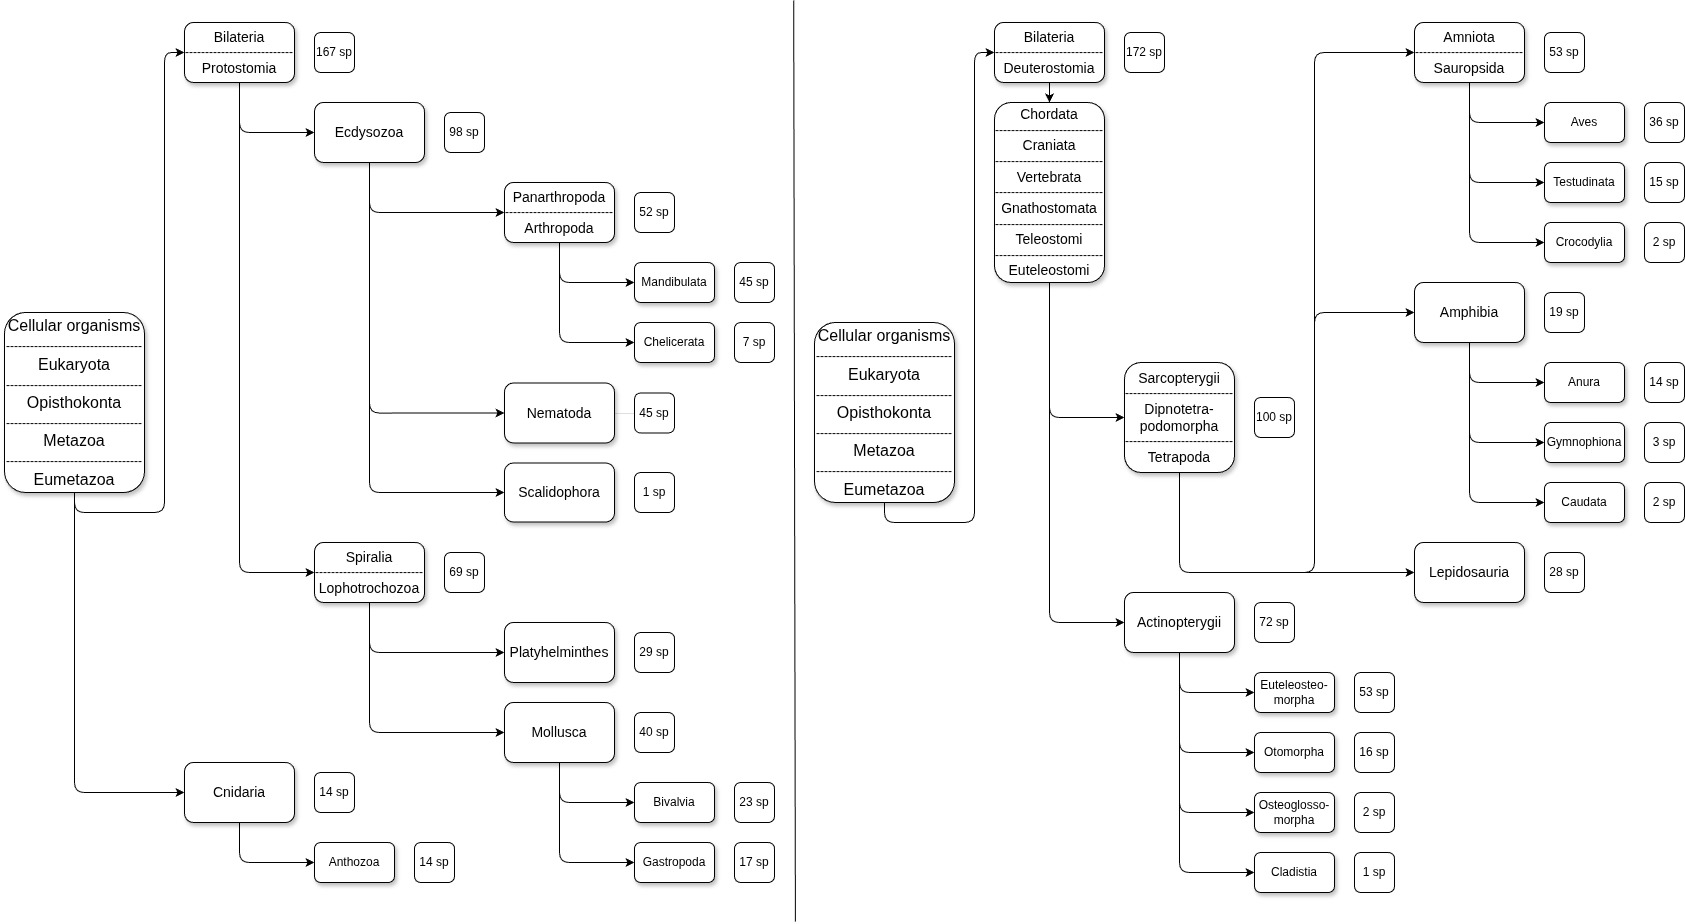
\includegraphics[width=1.0\textwidth]{images/Tree_summary}
    \caption{Количество видов, взятых в анализ для Protostomia+Cnidaria и Deuterostomia.}
    \label{fig:tree_1}
\end{figure}

\newpage
\begin{figure}[h] % here, top, bottom, page
    \centering
    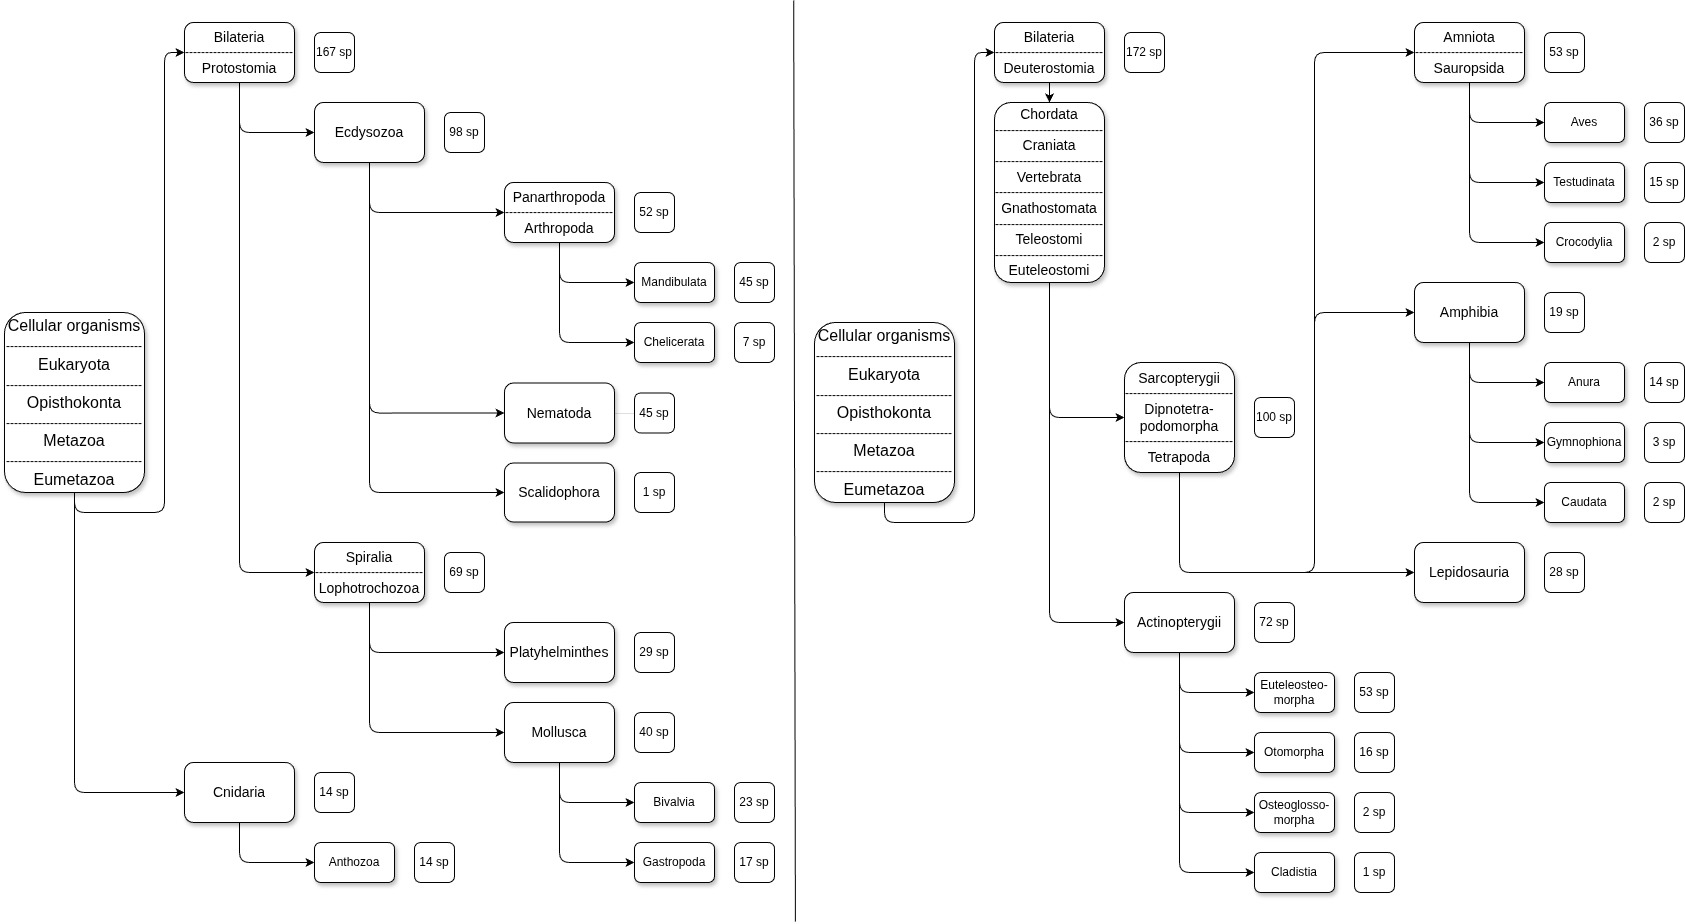
\includegraphics[width=1.0\textwidth]{images/Tree_summary_v2}
    \caption{Количество видов, взятых в анализ для Protostomia+Cnidaria и Deuterostomia.}
    \label{fig:tree_2}
\end{figure}

\newpage
\begin{figure}[h] % here, top, bottom, page
    \centering
    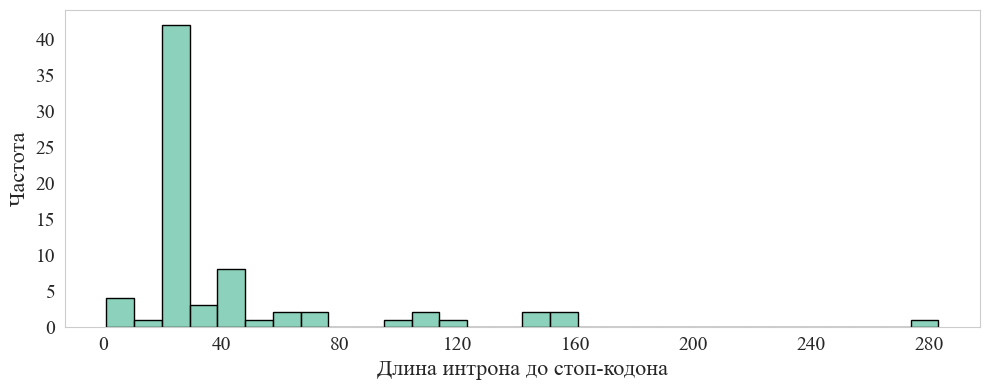
\includegraphics[width=1.0\textwidth]{images/Actinopterygii_intron_stop}
    \caption{Распределение длин части кассетного интрона до стоп-кодона у таксономической группы Actinopterygii}
    \label{fig:Actinopterygii_intron_stop}
\end{figure}

\newpage
\begin{figure}[h] % here, top, bottom, page
    \centering
    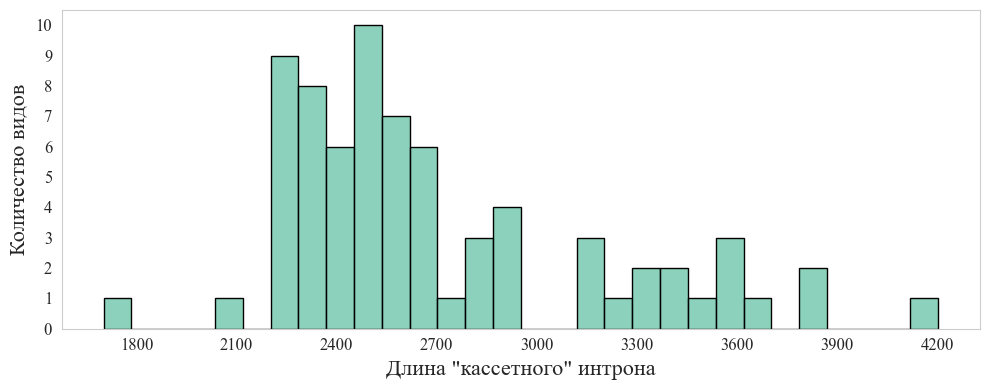
\includegraphics[width=1.0\textwidth]{images/Actinopterygii_intron}
    \caption{Распределение длин кассетного интрона у таксономической группы Actinopterygii}
    \label{fig:Actinopterygii_intron}
\end{figure}


% Список литературы
\newpage
\section{Список литературы}
\printbibliography[heading=none]


% Благодарности
% \clearpage
\section{Благодарности}

Я хотел бы поблагодарить моего научного руководителя, Голубкову Елену Валерьевну, и моего куратора, Бондарука Дмитрия Денисовича, за постоянную поддержку и помощь в обсуждении результатов работы.

Отдельно я хотел бы поблагодарить Абрамсон Наталью Иосифовну за повторное рецензирование работы моего авторства.

Также хочу выразить благодарность преподавателям программы ``Биоинформатика`` и кафедры генетики и биотехнологии СПбГУ, и коллективу преподавателей и ассистентов Института Биоинформатики за полученные знания в процессе обучения, с помощью которых стало возможным осуществление данной работы.

% Приложение (может быть пустым)
% \clearpage
\section{Приложение}



\end{document}
